
%(BEGIN_QUESTION)
% Copyright 2012, Tony R. Kuphaldt, released under the Creative Commons Attribution License (v 1.0)
% This means you may do almost anything with this work of mine, so long as you give me proper credit

How much work is done pumping 3,000 gallons of water from reservoir ``A'' to reservoir ``B'' over the hill?

$$\includegraphics[width=15.5cm]{i02613x01.eps}$$

If the pump's power output is 250 horsepower, how long will it take to pump all 3000 gallons to reservoir ``B''?

\vskip 20pt \vbox{\hrule \hbox{\strut \vrule{} {\bf Suggestions for Socratic discussion} \vrule} \hrule}

\begin{itemize}
\item{} Calculate the amount of pressure at the discharge port of the pump as it lifts water up to reservoir ``B''
\end{itemize}

\underbar{file i02613}
%(END_QUESTION)





%(BEGIN_ANSWER)

First, let's determine the weight of 3,000 gallons of water:

$$\left( 3000 \hbox{ gal} \over 1 \right) \left(231 \hbox{ in}^3 \over 1 \hbox{ gal} \right) \left(1 \hbox{ ft}^3 \over 1728 \hbox{ in}^3 \right) \left(62.4 \hbox{ lb} \over \hbox{ ft}^3 \right) = 25025 \hbox{ lb of water in 3000 gallons}$$

This weight of water will have to be lifted to the peak of the hill through the 100 foot pipe, but we will not use the figure of 100 feet as the displacement, since it is not vertical.  Instead, we will use trigonometry to calculate the vertical lift ($x$):

$$x = (100 \hbox{ ft})(\sin 48^o) = 74.31 \hbox{ ft vertical lift}$$

So, the work involved with lifting this much water to that height is:

$$W = F x \cos \theta$$

$$W = (25025 \hbox{ lb}) (74.31 \hbox{ ft}) \cos 0^o$$

$$W = 1,859,719.9 \hbox{ ft-lb of work}$$

Barring any piping friction, the horizontal section of pipe (55 ft) does not necessitate any work being done.  The short, 20 foot section of downward-angled pipe, however, actually {\it releases} energy (performs negative work) because it lets the water drop in height.  This drop is:

$$\hbox{drop} = (20 \hbox{ ft})(\sin 30^o) = 10 \hbox{ ft}$$

Since the same amount of water will drop this amount, the negative work done here is:

$$W = F x \cos \theta$$

$$W = (25025 \hbox{ lb}) (10 \hbox{ ft}) \cos 180^o$$

$$W = -250,250 \hbox{ ft-lb of work}$$

The total (net) work done, then, is the sum of these two figures:

$$W_{net} = 1,859,719.9 \hbox{ ft-lb} - 250,250 \hbox{ ft-lb} = 1,609,469.9 \hbox{ ft-lb of work}$$

\vskip 10pt

At a pump power output of 250 HP (137,500 ft-lb per second)

$$t = {W \over P}$$

$$t = {1609469.9 \hbox{ ft-lb} \over 137500 \hbox{ ft-lb/s}} = 11.71 \hbox{ seconds}$$

%(END_ANSWER)





%(BEGIN_NOTES)


%INDEX% Physics, energy, work, power

%(END_NOTES)


